\chapter{Background}
\label{chaBackground}
This chapter gives a brief introduction to programming languages and programming language theory -- though not nearly as comprehensive as a good book on the subject. Typechecking and type inference is also discussed. A birdseye view of computer-hardware and FPGA design is also given, for example what exactly is meant by wordlength.

% Programming languages in general is considered one of the more mature topics in computer science. There are many, many books and papers written on compilers. Some programmers even consider compilers to be black boxes which they must obey, frightened of the complexities and details of the black magic working inside. This background aims to unbox these beasts called compilers and shed some light on them. Explaining all the details of a compiler and the type checker is out of scope for this background.
% 
% Wordlengths, HDLs and also get a section describing how they fit into this work.


\section{Introduction to Compiler Structure}
What constitutes a compiler is not always obvious. A compiler, in the most banal sense, takes an input program and outputs an output program. Some want the output to be ``simpler`` than the input, passing in a high level program in C and outputting executable X86 machine code where X86 is considered a ``simpler`` than C. The input to the compiler is often text, and we will assume this for the rest of this short introduction to compilers.

Each compiler is unique, but they often have a shared structure. The first step is often to do lexical analysis (also called lexing) in a lexer or tokenizer. Here characters are abstracted away, and the compiler has done the first processing of the text. When lexing you often decide what piece of text is an integer-constant, a keyword, a string, etc. After the lexing the tokens are used to perform semantic analysis -- parsing. During parsing the compiler understands structures in the program such as what is part of each function or correctly parsing the order of operations for mathematical expressions. The parsing usually produces an abstract syntax tree (AST). Though some compilers interweave these steps, they are usually there in spirit.

The Spade compiler has both a lexer step and a parser step which are located in different modules.

The compilers work is not done yet. After all the syntactical analysis the semantic analysis can be started, semantic analysis is sometimes referred to as the ``inner layers of the compiler``. Here we resolve identifiers, run type-checking and other static program analysis or do optimizations like moving around constants to avoid needless copies. The wordlength inference and optimizations will be an inner layer, the relevant details will be discussed in the Section \ref{sec:TypeChecking}. 

After the compiler has finished optimizing, the output is generated and potentially lowered (made less complex) in multiple stages, often by translating to a simpler internal representation which in the end makes generating the final output of the compiler easier.

One ``layer`` is often called a ``pass``. Spade is not a multi-pass compiler and perform these steps sequentially -- not interleaved.
\cite{src:DragonBook}\cite{src:CraftingInterp}\cite{src:KKLectures}

\begin{figure}
\begin{center}
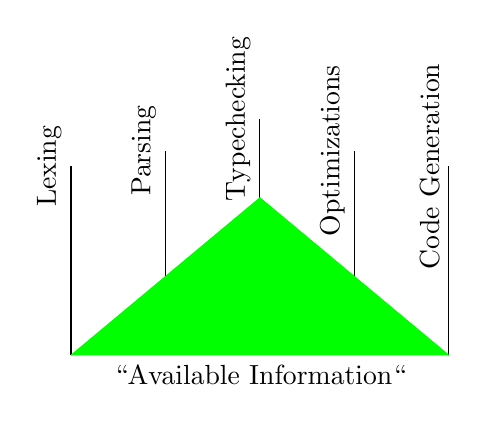
\begin{tikzpicture}[xscale=3, yscale=2]
% vertical lines
\draw (0,0) -- (0,1.2) node[above, rotate=90] {Lexing};
\draw (0.4,0) -- (0.4,1.3) node[above, rotate=90] {Parsing};
\draw (0.8,0) -- (0.8,1.5) node[above, rotate=90] {Typechecking};
\draw (1.2,0) -- (1.2,1.3) node[above, rotate=90] {Optimizations};
\draw (1.6,0) -- (1.6,1.2) node[above, rotate=90] {Code Generation};
% horizontal line
\filldraw[color=green, fill=green] (0,0) -- (0.8,1.0) -- (1.6,0);
\draw (0.8,0.0) node[below] {``Available Information``};
\end{tikzpicture}
  \caption{A visualization of the rough measurement of information present in each step of the compilation process. Typechecking having the most information and lexing and code generation having the least amount of information.}
  \label{fig:InformationCompilation}
\end{center}
\end{figure}

Compilers have to construct a lot of complex information about the program. A visual some find helpful when reasoning about compilers is an imagined graph of ``available information``. Figure \ref{fig:InformationCompilation} tries to communicate the amount of information created in each step of compilation. The most important part being that we know a lot about the program in the type checking phase.

\subsection{Abstract Syntax Tree}
General purpose programming languages need to be recursive in their structure -- one might want a sub-expression inside another expression for example. Representing this structure inside a computer cannot simply be done with a simple list of values, the data-structures themselves must reflect the structure of the language. One very popular way of storing this recursive syntactical information is by using an abstract syntax tree (often referred to as an AST). An AST describes the structure of the program.


\begin{figure}
\centering
\begin{subfigure}{.5\textwidth}
\begin{verbatim}
<expr> ::= <num>
         | <expr> + <expr>

<num>  ::= 0 | 1 | 2 | 3 | 4
\end{verbatim}
\end{subfigure}
  \caption{A simple BNF-like syntax-definition for integer expressions.}
  \label{fig:bnfExpr}
\end{figure}
For example, consider the grammar for integer addition expressions described in this psuedo-BNF format shown in Figure \ref{fig:bnfExpr}. The syntax understands whole numbers and the basic arithmetic operations addition (\verb!+!) and subtraction (\verb!-!). Most notable is that the syntax is recursive and expressions can contain expressions in themselves. This BNF-like syntax is a bit simplified and the grammar is not necessarily in a good format. A better grammar would handle order of operations and avoid ambiguities -- which will be explained later.

We can write a simple ''program'' that is a part of the language described by Figure \ref{fig:bnfExpr}. Some small valid ''programs'' are: \verb+1+, and \verb!1 + 1!. But we will focus on the more complex example in Figure \ref{fig:progExpr} -- which shows two additions.

\begin{figure}
\centering
\begin{subfigure}{.5\textwidth}
\begin{verbatim}
1 + 2 + 3
\end{verbatim}
\end{subfigure}
  \caption{A simple integer expression in the simple integer expression language with 3 terms and 2 additions.}
  \label{fig:progExpr}
\end{figure}

Looking at Figure \ref{fig:progExpr} it is obvious that the expressions should evaluate to 6. What is not obvious is how a computer should evaluate this expression. We can namely construct two different abstract syntax trees (and two different parse trees) for the program in Figure  \ref{fig:progExpr}. When parsing the program to a syntax tree we have to make the conscious decisions of what node is placed on top.


\begin{figure}
\centering
\begin{subfigure}{.5\textwidth}
\centering
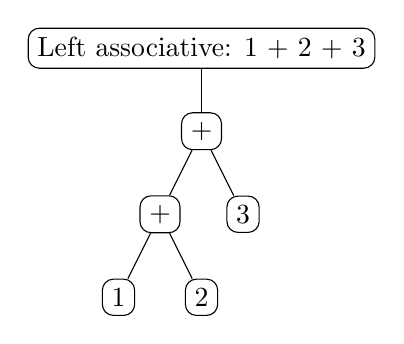
\begin{tikzpicture}[
  sibling distance=3em,
  level distance=3em,
  every node/.style = {shape=rectangle, rounded corners, draw, align=center}
]
  \node {Left associative: 1 + 2 + 3}
          child {node {+}
            child {node {+}
              child {node {1}}
              child {node {2}}
            }
            child {node {3}}
          };
\end{tikzpicture}
\end{subfigure}%
\begin{subfigure}{.5\textwidth}
\centering
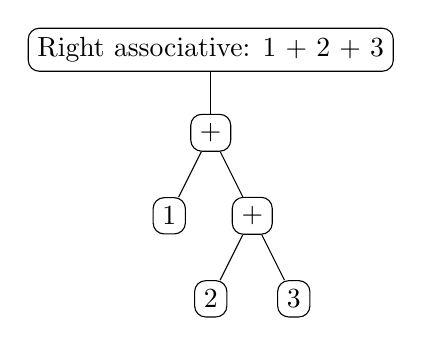
\begin{tikzpicture}[
  sibling distance=3em,
  level distance=3em,
  every node/.style = {shape=rectangle, rounded corners, draw, align=center}
]
  \node {Right associative: 1 + 2 + 3}
          child {node {+}
            child {node {1}}
            child {node {+}
              child {node {2}}
              child {node {3}}
            }
          };
\end{tikzpicture}
\end{subfigure}
  \caption{Two example syntax tree -- illustrating ambiguity in the grammar and the difference between left and right associativity.}
  \label{fig:astExpr}
\end{figure}

The Figure \ref{fig:astExpr} shows the two different associativities that causes \verb!1 + 2 + 3! to be interpreted as either \verb!(1 + (2 + 3))! or \verb!((1 + 2) + 3)!. For the observant reader there is not much difference between these mathematical expressions -- they are even considered equivalent since addition is associative for integers. The associativity property is unfortunately very rare in the real world of effectfull-programming. If evaluating an expression in this language was effectfull -- for example the result was printed, these different associativities would have different outputs. One of the programs would print \verb+1 2 3 3 6+ while the other would print \verb+1 2 3 5 6+ (ofcourse dependent on how the expressions are evaluated). This is what is called an ambiguity -- and an abstract syntax tree makes it clear how the compiler internally understands this addition.

There are different operations which can be done to an abstract syntax tree. In our very simple example of integer additions it would make sense to fold the constants and replace the entire AST with the constant 6 -- but to do that we would have to know the associativity of the \verb!+!-operator.

The AST is a very popular format to output from the parsing stage, since it is flexible. In the Spade-compiler the AST is annotated with type information as it is discovered -- this annotated AST is then feed either to a language server or a code generation phase.

\section{Type Checking} % Maybe `inner layers`?
\label{sec:TypeChecking}
Type checking is a way of making sure the program is internally consistent, there are no contradictions inside to program to the program itself. Type checking can be done in different ways with different pros, cons or preferences \cite{src:TypeCheckersBook}. The type checker in Spade can infer types and deduce things about the program, like ``the first argument is a 3-bit integer value, but you gave a record`` \cite{src:spadeAnHDL}. Typechecking has shown to reduce some kinds of programming errors and can in some cases even suggest what functions to use.

The type checker in Spade is a one directional Damas–Hindley–Milner typechecker. This means it stops on the first error and can deduce types to their most general form. So if asked to type check the identity function (a function that takes one value and returns the value as is, the function does nothing) the type checker would be able to deduce that the argument could have any type, but that the type is the same as the return value, without any help from the programmer except the body of the function. \cite{src:DamasHindleyMilner}

There is also a connected topic of type inference -- a program that guesses the types of expressions based on the context. A sufficiently good typeinferer could be used to check the types of the program and can easily be modded into a typechecker. It is infact upon this idea that the Damas–Hindley–Milner typechecker works. In this paper, we will freely refer to typecheckers and work by typeinference as both typecheckers and typeinferrence -- even though it might not be the most correct according to the literature we deem it adds variety and clarity to how these systems function.

\subsection{Unification}
A Damas-Hindley-Milner typechecker is a very simple typechecker and is based upon one simple idea -- typeinference is a constraint satisfaction problem with \textbf{only} equivalence-constraints. The idea of the typechecking and typeinference is to simply find types that has to be equal for the program to function. Most of these small rules are painfully simple -- like: ''adding two numbers gives you a number'', or ''calling a function results in a type with the return value of the called function''. What really drives these simple rules is a process called unification. Unification is a way to propagate these equality constraints. This is proved to be correct, given that all expressions without sub-expressions have a type.

This unification property is also found in logic-programming, which is not a coincidence but rather an effect of the Curry–Howard isomorphism. \cite{src:curryHowardIso}

I find examples useful to quickly get basic understanding of a topic, so I will outline the typechecking of a simple program and how the unification step would work. We will typecheck the simple program in Figure \ref{fig:progUni}.

\begin{figure}
\centering
  \begin{subfigure}{.5\textwidth}
\begin{verbatim}
fn add<A> : (A, A) -> A

fn main { add(add(1, 2), "abc") }
\end{verbatim}
  \end{subfigure}
  \caption{A simple dummy program to show unification. A simple ''add'' function is defined which takes 2 arguments of the same type and returns that type. Types are denoted with uppercase letters and language constructs are defined using lowercase letters.}
  \label{fig:progUni}
\end{figure}

Let us assume that we have two types in our language \verb+Int+ and \verb+Str+. We start by giving each construction a unique type variable (this is mainly to make it simple to explain, there are more resource efficient ways of accomplishing this). We then evaluate the syntax tree bottom upp. We will also assume the rules: (1) integer-constants have the type \verb+Int+, (2) String-constants have the type \verb+Str+, (3) Calling a function means the types of the arguments and parameters are the same and the whole expressions evaluates to the return type of the function. Evaluating rule (3) always gives a new type ''A'', we will keep track of these with numbered suffixes. These 3 simple rules let us typecheck and typeinfer the expression in the main-function.

In this explanation the \verb+:+ operator denotes that an expression on the left has a known type on the right, so \verb+1:Int+ means the expressions \verb+1+ has type \verb+Int+. We will also denote the unifications of types, so \verb+A9=A8+ means the type \verb+A9+ is the same types as \verb+A8+. We first of all know the type of all the simple expressions -- thanks to rules (1) and (2) -- that means \verb+1:Int+, \verb+2:Int+ and \verb+"abc":Str+. We can now solve \verb+add(1, 2)+ by applying rule (3) to \verb+add:(A0, A0) -> A0+ and \verb+add(1, 2):T1+, we can unify \verb+(Int, Int)+ and \verb+(A0, A0)+, which gives \verb+A0=Int+. We also get \verb+T1=A0=Int+ which gives us \verb+add(1, 2):Int+. The more complex expression is now inferable \verb+add(add(1, 2), "abc"):T2+, we unify \verb+(T1, Str)+ and \verb+(A1, A1)+ which gives us a contradiction, since \verb+T1=Int=/=Str+ -- this would result in a type error which might throw an error.

In conclusion, unification lets us define two types as the same type and send all this information as far as we want in a program -- there are programming languages with global type-inference for example. But the method described by Damas-Hindley-Milner is limited to equality-constraints which has some limitations in what types can be expressed.

\subsection{Monomorphisation}
After all the typechecking and typeinference has been done, something called monmorphisation is done. This phase make generic functions into concrete function -- that is to say all functions with generics like \verb+fn add<A>(x: A, y: A) -> A+ are given concrete types like \verb+fn add(x: i32, y: i32) -> i32+. This means the same code can lead to multiple function bodies. Monomorphisation creates a new instance of a function for each of the generic arguments given, and Rust does something similar. \cite{src:rustMono}

Monomorphisation is often considered a performance optimization, but for HDLs this step is absolutely required.

\section{Interval Arithmetic, Affine Arithmetic and Self Validating Numerical Methods}
\label{sec:IAndAA}

There is an excellent explanation of both Interval- and Affine Arithmetic by \citeauthor{src:affAri} -- the following section is a short version to cover the absolute basics of the material.

Affine arithmetic and interval arithmetic and two common ways to estimate. They can be applied to estimate bounds for mathematical functions or things that can be modeled by mathematical functions. They also have a place in static analysis of programs, which is the focuses of this thesis. This section describes what these concepts are, references literature if you want to read more and shows their roll in static analysis of programs. These methods are often referred to as over-estimation.

Though affine arithmetic is more sophisticated it does not always produce better results, interval arithmetic can for some computations produce tighter bounds. There are other methods for overestimation that are considered more sophisticated like ME-gPC \cite{src:MEgPC} and modified affine arithmetic, but the extra complexity can be added later if it is found to be needed. ME-gPC was not considered for this thesis due to its complexity -- but it is a good extension to the techniques explained in this paper. Affine arithmetic and interval arithmetic are the simplest methods that offer enough complexity to be interesting.

\subsection{Interval Arithmetic}
Interval arithmetic operates on intervals, as the name implies. A value -- or in the context of a program, a variable -- has a smallest and largest value it can assume. Consider \verb`x = random_real()`, where \verb`random_real` generates a random value in the range $[0, 1]$. We can express this in interval arithmetic as $\bar{x} = [0, 1]$, intervals will be denoted with a bar on top to separate them from the variables. Note especially that the true value of $x$ lies in the interval $\bar{x}$. In this example we know $0 \leq x \leq 1$, also written as $x \in [0, 1]$. These intervals can be added, negated, and so on, to give you an estimate of an arbitrary expression.

For a more throughout guide on implementations \citetitle{src:affAri} by \citeauthor{src:affAri} is worth your time, this section will cover the basics that are needed to understand the concept and understand this thesis. A full description of the field is out of scope.
\subsubsection{Interval Arithmetic Special values}
When doing static program analysis, some extra values are often defined. For example, it is okay to have an interval where one value is infinite. This interval $[5, \infty]$ is perfectly valid.

The empty interval is also defined and written as $[]$. The empty interval usually denotes expressions or code that cannot be reached or evaluated. It might seem useless at a glance, but is required to do more sophisticated static analysis.

\subsubsection{Interval Arithmetic: An example and Limitations}
Examples are often helpful.
We will be using the expression $2x + z - z$ as an example where $x = [0, 1], z = [1, 3]$.

\begin{verbatim}
2 * [0, 1] + [1, 3] - [1, 3]
// Scaling rule and subtraction is negated addition 
[2 * 0, 2 * 1] + [1, 3] + (-1 * [1, 3])
// Calculate
[0, 2] + [1, 3] + [-3, -1]
// Sum it upp
[-2, 4]
\end{verbatim}

This gives us the conclusion that this expression will lie in the range $[-2, 4]$ for the given values of $x$ and $z$. This is true, but the estimate is larger than it necessarily needs to be. An observant reader would notice that subtracting the value $z$ from itself should result in $0$, which is a perfectly valid point. This is a limitation of the interval arithmetic. Interval arithmetic does not reason about the expressions that came before it and how they combine, and this limitation would exist if used to do static analysis of programs. This limitation leads us to affine arithmetic which understands the relations between variables we evaluate. Affine arithmetic can more accurately calculate expressions like $a - a$ since it understands that $a$ and $a$ is the same thing.

\subsection{Affine Arithmetic}
Affine arithmetic (AA) works similarly to interval arithmetic (IA), but has a memory of where values come from and can reason about their combinations at a higher level. That said, AA does not produce strictly better results than IA in all circumstances and a combination is currently thought to be the current state of the art. \cite{src:affAri}

\subsubsection{How Affine Arithmetic works}
In affine arithmetic there is a concept of noise symbols ($e_i$ where $i$ is a natural number) and the numbers half width ($x_i$ where $i$ is a natural number). A linear combination of these noise symbols is a reasonable way to represent a "number" when reasoning about affine arithmetic, $\hat{x} = x_0 + x_1e_1 + x_2e_2 + \dots$. These terms can them be combined using similar rules to interval arithmetic. \cite{src:affAri}

Notice how the first term lacks a noise symbol, this expresses where the center of the uncertainty is. The different noise variables serve as the memory of this expression, consider subtracting $\hat{x} - \hat{x}$ with itself we get the expected result of 0 from that.

\subsection{When Interval Arithmetic Is Better Than Affine Arithmetic}
Affine arithmetic may seam like the superior option in all cases -- this is not the case. Affine arithmetic has trouble with multiplication, and has to add extra noise in order to constantly overestimate. This extra noise is particularly relevant when handling large expressions. Interval arithmetic can fair a lot better here since multiplication does not add noise in the same way. One very concrete example is if all variables in an expression like $\prod x_i$ are in the range $[0,n)$ -- affine arithmetic does not respect $0$ in the same way and would give us a range poking out below $0$ while interval arithmetic would correctly infer the lower bound of $0$.

When concerned with estimating arithmetic expressions we can both get the pie and eat it. Since both interval arithmetic and affine arithmetic offer estimates which are too large, we can take the subset of the guesses and be sure of the correctness.

\subsection{Error Explosion for Affine- and Interval Arithmetic}
\label{sec:ee}
Both affine arithmetic and interval arithmetic compensate for unknown factors with a span of potential values. This method is fine for most computations that are small and simple, but this isn't always the case. Some calculations result in large spans of potential values -- since a smaller span gives more certainty and are easier to account for.
\cite{src:affAri}

\section{Wordlength Inference and Typechecking in Spade}
\label{sec:TheProblem}
Most values in Spade take up bits or space in the run time environment. Wordlength inference is mostly concerned with numbers -- so consider positive numbers without a decimal. Consider a program with a counter that resets to 0 after counting to 3, we do not need 32 bits to represent it. The cost of storing a number with 32 bits compared to 2 bits could be large if it requires a larger FPGA, extra circuit components or a different power rating. Compared to software where memory is considered abundant -- this causes Spade as a HDL to be designed differently compared to a highlevel programming language.

Wordlength inference is the compiler understanding what wordlength -- the number of bits -- is needed to store a value. Inferring this value well causes good resource usage and requires less manual intervention. Doing it poorly or not at all either requires users to manually specify the wordlength of each value, or a hardware that is inefficient.

\begin{figure}[h]
\begin{center}
\begin{verbatim}
fn f(a: int<3>) -> int<4> {
  a + 1 + 1
}

entity main(clk: clock, rst: bool) -> int<4> {
  f(3)
}
\end{verbatim}
\end{center}
\label{fig:SimpleFaultSpade}
\caption{``simple\_fault.spade`` A simple spade program that does not compile, showing the current limitations of wordlength inference.}
\end{figure}

\begin{figure}[h]
\begin{center}
\begin{verbatim}
error: Type error
  ┌─ src/simple\_fault.spade:1:27
  │
1 │   fn f(a: int<3>) -> int<4> {
  │                      ------ int<4> type specified here
  │ ╭───────────────────────────^
2 │ │   a + 1 + 1
3 │ │ }
  │ ╰─^ Found type int<5>
  │
  = Expected: 4
  =       in: int<4>
  =      Got: 5
  =       in: int<5>

Error: aborting due to previous error
\end{verbatim}
\end{center}
\label{fig:SimpleFaultSpadeCompileOutput}
\caption{The output from the compiler when trying to compile the program ``simple\_fault.spade``}
\end{figure}

Consider the program in Figure \ref{fig:SimpleFaultSpade}. The function ``f`` adds 3 values together, two of which are known constants. We also know that $2^3 + 2 < 2^4$ -- we should be able to fit the result of the addition into the 4 bit word without loss of data. The compiler does not agree as seen in the compiler output in Figure \ref{fig:SimpleFaultSpadeCompileOutput} where it claims we need 5 bits to store this value. This problem might seem inconsequential since calculating constant expressions during compilation would fix this, as seen by the program in Figure \ref{fig:SimpleCorrectSpade} compiling without worries. Only fixing this problem for constants would be nice variables would cause the same problem to appear but in a more difficult form. The problem here is much deeper, and is a direct cause of the typechecking algorithm itself.

\begin{figure}[h]
\begin{center}
\begin{verbatim}
fn f(a: int<3>) -> int<4> {
  a + 2
}

entity main(clk: clock, rst: bool) -> int<4> {
  f(3)
}
\end{verbatim}
\end{center}
\label{fig:SimpleCorrectSpade}
\caption{``simple\_correct.spade`` A spade program that does compile, which is very similar to the program in Figure \ref{fig:SimpleFaultSpade}}
\end{figure}

The Spade compiler implements a the Damas-Hindley–Milner typechecker -- discussed in more detail in Section \ref{sec:TypeChecking}. Damas-Hindley-Milner runs in almost linear time (if implemented correctly) but is not complete. The completeness property for type checkers means there are programs which are correct but that the type checker will not recognize as correct. The programs from Figures \ref{fig:SimpleFaultSpade} and \ref{fig:SimpleCorrectSpade} are an example of this. This observation is important since it means this is not a bug, but a limitation of the compiler itself. How this should be changed and to what is the central topic of this thesis.

\section{Field Programmable Gate Array}
A field programmable gate array (FPGA) is a kind of programmable hardware. An FPGA is slower and draw more power than a ''normal'' circuit but FPGAs allow very fast iteration since they are programmable. This makes FPGAs ideal for prototyping hardware designs. An FPGA is made up of a grid of components all connected by busses -- each component can then be programmed and connected individually. \cite{src:FPGA}

An FPGA is very different from a general purpose computer or CPU which is what is mostly programmed by highlevel languages. An FPGA is a circuit which means all steps are taken simultaneously -- this allows massive parallelism since each part of the circuit has to complete before the next iteration can be taken. This makes FPGAs ideal for things like realtime signal processing -- which is why they see a lot of use in media processing and military applications \cite{src:FPGAApplications}. These physical limitations also put restrictions on the HDL. This is why state (except memories) is immutable in Spade.

\subsection{Place and Route}
Place and Route, sometimes referred to as PNR in this thesis is when the program is encoded as hardware, which requires routing the information in the actual chip and deciding what node is responsible for what computation. This is similar to how the routes are placed on a ''normal'' circuit and is considered a computationally hard problem. Since the problem of PNR is computationally hard, a stochastic algorithm is applied, meaning the same program might not generate identical encoded hardware. When trying to measure the resource usage of FPGA programs this step needs to be run multiple times, since one run could always be a fluke.

\section{Spade}
Spade is a HDL taking a lot of inspiration from Rust to create a more modern HDL (Hardware Description Language). Spade has syntax which mimics that of Rust and tries to remove problems people have when using other HDLs like System Verilog. One of the biggest features of Spade is the static typechecking which allows programs to be verified before even being synthesized -- creating a faster iteration loop.
\cite{src:spadeSomething} \cite{src:spadeAnHDL}

\subsection{Swim}
The Spade-language has a build-tool call Swim. Swim orchestrates things like running PNR, running synthesis tools, installing dependencies, generating basic projects and compiling Spade-code. Swim is the best way to handle any Spade project.

